%%%%%%%%%%%%%%%%%%
% TODO: ARG-ASP-distance
%%%%%%%%%%%%%%%%%%
In this section the conformation of soluted FAK (FAK-SOL) for the \martini force field is investigated. Since the secondary structure of the two domains is fixed with the elastic network, the focus is on the FERM kinase interface.\\
\\
First the COM distances of F1 to the N-lobe ($d_\text{F1-N}$) and F2 to the C-lobe ($d_\text{F2-C}$) are considered. The two dimensional histogram of the distances reveals two different states ( \autoref{free:f2clf1nl}). Spot 1 refers to conformations, which are partially opened at the F2 - C-lobe interface, but close at the F1 - N-lobe interface. In contrast to this the conformations of spot 2 refers to states, in which F2 and the C-lobe gets closer while the distance between F1 and the N-lobe is increased. During the simulation several transitions between the spots were obtained, which indicates no convergence to a preferred spot. However, there is only a minor effect upon the contact area (\autoref{free:ca}).  Spot 2 show a slightly larger mean of $27.6\,\si{\nano\metre}^2$ in comparison to spot 1 ($27.1\,\si{\nano\metre}^2$).\\
\\
%
%
%
\begin{figure}
	\subcaptionbox{\label{free:f2clf1nl}}[0.49\textwidth]{
		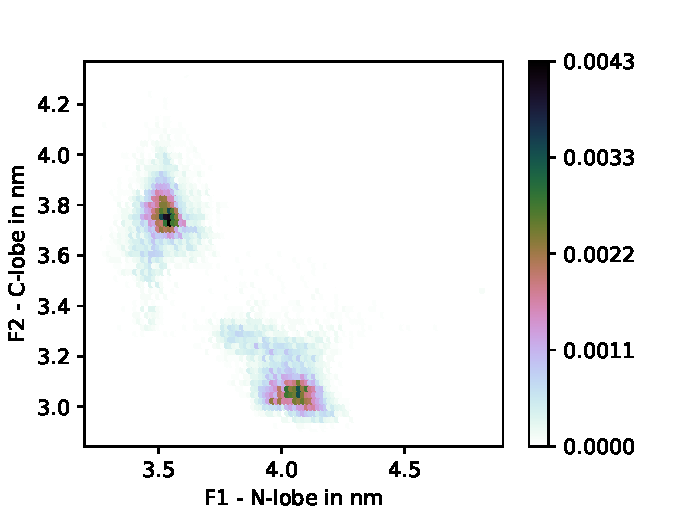
\includegraphics[height=5cm]{figures/results/free_f1f2}
	}\hfill%
	\subcaptionbox{\label{free:ca}}[0.49\textwidth]{
		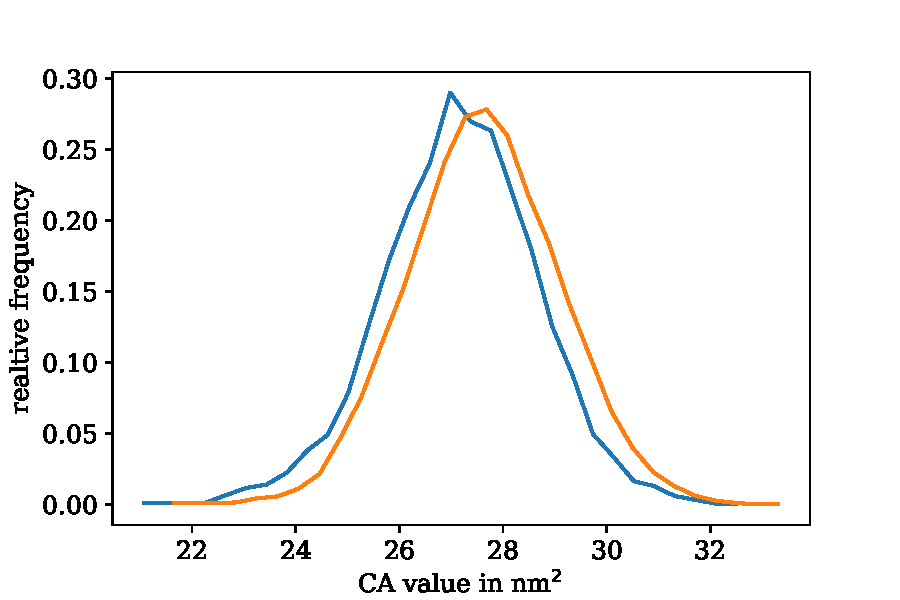
\includegraphics[height=5cm]{figures/results/free_ca}
	}%
	\nicecaption{Domain distances and contact area of FAK-SOL}{(\subref{free:f2clf1nl}): two dimensional, normed histogram of $d_\text{F1-N}$ and $d_\text{F2-C}$. (\subref{free:ca}): distribution of CA}
\end{figure}
%
%
%
A contact map of the interface between the FERM domain and the kinase for frames of spot 2 can be found in \autoref{free:contact}. Two contact areas can be identified at the FERM-kinase interface. The first one (area 1) is located between F1 and the N-lobe/activation loop. It shows i.e. contacts between \acid{Y}{576} and \acid{Y}{577} and residues of the FERM domain. The minimal distance in this area, occurring between residue \acid{H}{41} and \acid{Y}{576}, is $0.45\,\si{\nano\metre}$ with an RMSF value of $0.03\,\si{\nano\metre}$. This area reflects the burying of the activity regulating residues in closed state.\\
The second contact area (area 2) is located between F2 and the C-lobe. The spots occur around the residues \acid{Y}{180} and \acid{D}{200} of F2 as well as \acid{F}{596} and \acid{R}{665} of the C-lobe. The minimal distance in this area occurs between \acid{Y}{180} and \acid{F}{596} with $0.45\,\si{\nano\metre}$ and an RMSF value of $0.02\,\si{\nano\metre}$. Mutation experiments showed, that these two residues have an important effect upon the interface \autocite{structFAK}, which fits to the obtained contact.\\
The linker show contacts with both domains. The minimal distances in the marked areas occur between the autophosphorylation site \acid{Y}{397} and \acid{H}{58} of F1 ($0.45\,\si{\nano\metre}$, RMSF $0.03\,\si{\nano\metre}$) as well as \acid{Y}{397} and \acid{Y}{576} of the kinase ($0.50\,\si{\nano\metre}$, RMSF $0.10\,\si{\nano\metre}$). These contacts support the thesis, that autophosphorylation is prevented in closed conformation by a binding of the linker to the FERM domain \autocite{pap003}.\\
% In contrast to \autoref{free:contact}, the contact map for frames of spot 1 show less contacts between F2 and the C-lobe, i.e. around the mentioned residues \acid{Y}{180} to \acid{M}{183}. A few additional contacts appear between F1 and the N-lobe, but these are only minor spots.
%
%
%
\begin{figure}
	\centering
	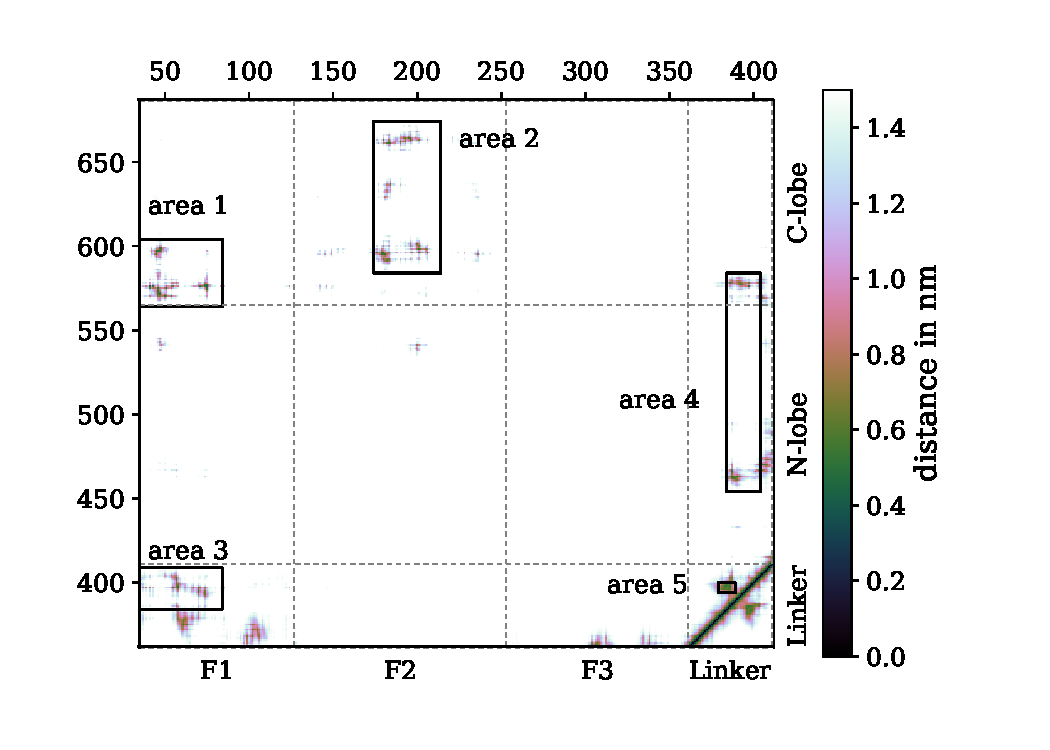
\includegraphics[width=.7\textwidth]{figures/results/contactmap_free}
	\captionof{figure}{Contactmap of interface between FERM domain and kinase}
	\label{free:contact}
\end{figure}
%
%
%
